\documentclass{extarticle}

% Файл: settings/pdflatex_notes.tex
% Основные настройки для документов LaTeX

% ========================================
% Пакеты сгруппированы по функционалу
% ========================================

% Основные настройки документа
\usepackage{geometry} % Настройки полей и страницы
\usepackage[T2A]{fontenc} % Кодировка шрифтов для кириллицы
\usepackage[utf8]{inputenc} % Кодировка текста
\usepackage[russian]{babel} % Поддержка русского языка
\usepackage{array}
\usepackage{indentfirst} % Красная строка
\usepackage{setspace} % Межстрочный интервал
\usepackage{ulem} % Подчеркивания

% Графика и оформление
\usepackage[most]{tcolorbox} % Стильные боксы
\usepackage{graphicx, wrapfig, caption, placeins} % Работа с изображениями
\usepackage{float} % Позиционирование рисунков
\usepackage{subcaption} % Подписи к подрисункам
\usepackage{booktabs} % Профессиональные таблицы
\usepackage{longtable} % Длинные таблицы

% Математика
\usepackage{amsmath, amssymb, amsfonts, mathtools, commath, cancel}
\usepackage{bm} % Жирные математические символы
\usepackage{nicefrac} % Красивые дроби

% Заголовки и колонтитулы
\usepackage{titlesec} % Стили заголовков
\usepackage{fancyhdr} % Колонтитулы
\usepackage{abraces} % Фигурные скобки

% Гиперссылки (должен быть загружен последним!)
\usepackage{hyperref}
\usepackage{xurl} % Для переноса длинных URL
\usepackage{tikz}
\usetikzlibrary{shapes, arrows.meta, positioning}

% Основной размер шрифта и межстрочный интервал
\renewcommand{\normalsize}{\fontsize{12pt}{14pt}\selectfont} % 12pt - размер, 14pt - межстрочный интервал

% ========================================
% Основные настройки
% ========================================

% Шрифты
\renewcommand{\rmdefault}{cmr} % Основной шрифт (Computer Modern)
\renewcommand{\sfdefault}{cmss} % Без засечек
\renewcommand{\ttdefault}{cmtt} % Моноширинный

% Абзацные отступы и интервалы
\setlength{\parindent}{1.5em} % Абзацный отступ
\setlength{\parskip}{0.5em} % Интервал между абзацами

% Настройка geometry
\geometry{
	a5paper,
	left=10mm,
	right=10mm,
	top=5mm,
	bottom=10mm,
	headheight=10mm,
	headsep=4mm,
	footskip=10mm,
	includeheadfoot
}

% Стили заголовков
\titleformat{\section}[block]{\bfseries\centering\newpage\huge}{\thesection.}{0.5em}{}[]
\titleformat{\subsection}[block]{\bfseries\centering}{\thesubsection.}{0.5em}{}[]
\titleformat{\subsubsection}[block]{\bfseries\centering}{}{0.5em}{}[]

% Настройка колонтитулов
\pagestyle{fancy}
\renewcommand{\headrulewidth}{1pt}
\fancyhead{}
\fancyhead[L]{\nouppercase{\leftmark}}
\fancyfoot[C]{\thepage}
\fancyfoot[R]{Скороходов С.А.}
\renewcommand{\sectionmark}[1]{}
\renewcommand{\subsectionmark}[1]{\markboth{#1}{}}

% Настройка математики
\numberwithin{equation}{subsection}
\mathtoolsset{showonlyrefs=false}

% Настройка изображений
\graphicspath{{./img/}}
\renewcommand{\figurename}{Рис.}
\captionsetup{labelsep=space}

% Гиперссылки
\hypersetup{
	colorlinks=true,
	linkcolor=blue,
	filecolor=magenta,
	urlcolor=cyan,
	pdftitle={Заметки},
	pdfpagemode=FullScreen,
}

% ========================================
% Пользовательские команды
% ========================================

% Блоки определений
\newtcolorbox{tbox}[2][]{
	colback=white!98!black,
	colframe=white!80!black,
	fonttitle=\bfseries,
	coltitle=black,
	title={#2},
	breakable,
	standard,
	before={\addcontentsline{toc}{subsubsection}{\protect\numberline{}#2}}
}

% Теоремы и определения
\usepackage{amsthm}

\theoremstyle{definition}
\newtheorem{definition}{Определение}[section]

\theoremstyle{plain}
\newtheorem{theorem}{\bfseries Теорема}
\newtheorem{corollary}[theorem]{Следствие}
\newtheorem*{proof*}{Доказательство}

\theoremstyle{remark}
\newtheorem{remark}{Замечание}[section]
\newtheorem{example}{Пример}[section]

% Удобные математические операторы
\DeclareMathOperator{\grad}{grad}
\DeclareMathOperator{\divergence}{div}
\DeclareMathOperator{\rot}{rot}

\usepackage{draftwatermark}
\usepackage{xfrac}
\SetWatermarkFontSize{10pt}  % Explicitly set reasonable size
\SetWatermarkScale{2.5}
\SetWatermarkLightness{0.9}
\SetWatermarkText{\textbf{Скороходов Сергей Александрович}}

\newcommand{\sumzerotoinf}{\sum\limits_{n=0}^{\infty}}
\newcommand{\sumonetoinf}{\sum\limits_{n=1}^{\infty}}
\newcommand{\N}{\mathbb{N}}
\newcommand{\R}{\mathbb{R}}

\newcommand{\nisum}{\sum\limits_{n = 1}^{\infty}}
\newcommand{\nzisum}{\sum\limits_{n = 0}^{\infty}}
\newcommand{\nilim}{\lim\limits_{n \to \infty}}

\newcommand{\nsum}[2]{\sum\limits_{n = #1}^{#2}}
\newcommand{\lint}[2]{\int\limits_{#1}^{#2}}




\begin{document}
	{\thispagestyle{empty}
\newgeometry{
	left=2cm,
	right=2cm,
	top=2cm,
	bottom=2cm
}
\begin{center}
	МИНИСТЕРСТВО НАУКИ И ВЫСШЕГО ОБРАЗОВАНИЯ РОССИЙСКОЙ
	ФЕДЕРАЦИИ\\

	\hfill \break
	Федеральное государственное автономное образовательное учреждение высшего образования «Национальный исследовательский Нижегородский государственный университет им. Н.И. Лобачевского» \\

	\hfill \break
	Радиофизический факультет\\
	\vspace{1.5cm}
	С. А. Скороходов\\
	\begin{center}
		{\huge \textbf{ОТВЕТЫ НА ФИЗИКУ}}
	\end{center}
	\hfill

	{Ответы на вопросы экзамена \\ Дисциплины -- Физика}\\
	\hfill

	Студента группы 417/0424С1ИБг1\\
	1 курса специалитета\\
	\hfill \break
	Основная образовательная программа\\
	подготовки по направлению\\
	10.05.02 «Информационная безопасность\\
	телекоммуникационных систем»\\
	(направленность «Системы подвижной цифровой\\
	защищенной связи»)
\end{center}

\vfill
\begin{center} Нижний Новгород \\ Издательство "Невыспавшийся Студент" \\ \the\year{} \end{center}
\thispagestyle{empty}
\newpage
}

	\tableofcontents
	\newpage
	\section{Ответы на вопросы}
	В данном разделе представлены ответы на все билеты по физике за 1 курс 2 семестра.

	\subsection*{Предупреждение}
	Данные ответы были составлены не самым умным студентом из-за чего могут встречаться различного рода ошибки. Просим сообщать о их нахождении по контактным данным, указанные в конце документа.

	\nopagebreak
	\subsection{\textbf{Теорема об изменении импульса с.м.т.} Условия сохранения импульса.}


	\subsection{\textbf{Теорема о движении центра масс.}}

Центр масс системы материальных точек называется геометрическая точка такая, что $\vec{r}$ которой равен:
\[\begin{aligned}
	\vec{r}_c = \frac{\sum_{i=1}^{n} m_i \vec{r}_i}{M} &&&& M = \sum_{i=1}^{n} m_i
\end{aligned}\]

Рассчитаем скорость центра масс:
\begin{multline*}
	\vec{v}_c = \dd{\vec{r}_c}{t} = \frac{1}{M} \dd{}{t} \Big(\sum_{i=1}^{n} m_i \vec{r}_{i}\Big) = \frac{1}{M} \sum_{i=1}^{n} m_i \vec{v}_i = \frac{\vec{p}}{M} \Rightarrow \boxed{\vec{p} = M \vec{v}_c}
\end{multline*}

Центру масс можно приписать импульс всей системы:
\begin{align*}
	\dd{\vec{p}}{t} = \vec{F}_{\text{внеш}} && \vec{p} = M\vec{v}_c \quad\to\quad M\vec{a}_c = \vec{F}
\end{align*}

\begin{tbox}{Замечания}
	\begin{enumerate}
		\item Расположение центра масс не зависит от выбора точки:
		\[\vec{r}_i = \vec{r}_i^{\,\prime} + \vec{\rho}\]
		\[\vec{r}_i = \frac{1}{M} \sum_{i=1}^{n} m_i \vec{r}_i = \frac{1}{M} \sum_{i=1}^n m_i \vec{r}_i^{\,\prime} + \frac{1}{M} \sum_{i=1}^{n} m_i \vec{\rho} = \vec{r}_i^{\,\prime} + \vec{\rho}\]
		\item Внутренние силы не влияют на движение центра масс. Они воздействуют на него, но опосредованно;
		\item Теорема о движении центра масс предоставляет общее представление о системе. Для более детального анализа систему переводят в систему отсчета, связанную с центром масс, и исследуют ее более подробно.
	\end{enumerate}
\end{tbox}
	\subsection{Уравнение Мещерского. Реактивная сила.}
	\subsection{\textbf{Теорема об изменении момента импульса с.м.т.} Закон сохранения момента импульса.}

\textbf{Момент импульса системы материальных точек} относительно начала координат $O$ — это сумма моментов импульса всех точек системы, взятых относительно того же начала $O$.

\[\vec{N} = \sum_{i=1}^{n} [\vec{r}_i; \, \vec{p}_i]\]
\begin{align*}
	&\dd{\vec{N}_1}{t} = [\vec{r}_1; \, \vec{f}_{21}] + \dots + [\vec{r}_i; \, \vec{f}_{i1}] + \dots + [\vec{r}_1; \, \vec{f}_{n1}] + [\vec{r}_1; \, \vec{F}_{1}] \\
	&\dd{\vec{N}_i}{t} = [\vec{r}_i; \, \vec{f}_{1i}] + \dots + [\vec{r}_i; \, \vec{f}_{i-1 \, i}] + [\vec{r}_i; \, \vec{f}_{i+1 \, i}] + \dots + [\vec{r}_i; \, \vec{f}_{ni}] + [\vec{r}_i; \, \vec{F}_{i}] \\
	&\dd{\vec{N}_n}{t} = [\vec{r}_n; \, \vec{f}_{1n}] + \dots + [\vec{r}_n; \, \vec{f}_{in}] + \dots + [\vec{r}_n; \, \vec{f}_{n-1 \, n}] + [\vec{r}_n; \, \vec{F}_{n}]
\end{align*}
\begin{align*}
	\sum_{i=1}^{n} \dd{\vec{N}_i}{t} = \sum_{i=1}^{n} [\vec{r}_i; \, \vec{F}_i] && \sum_{i=1}^{n} \dd{\vec{N}_i}{t} = \dd{}{t} \sum_{i=1}^{n} \vec{N}_i = \dd{\vec{N}}{t}
\end{align*}
	\subsection{\textbf{Теорема об изменении кинетической энергии с.м.т.}}
	\subsection{Потенциальная энергия с.м.т. \textbf{Теорема об изменении механической энергии с.м.т. Условия сохранения механической энергии.}}

\subsubsection*{Теорема об изменении механической энергии с.м.т.}
Запишем теорему для \textit{материальной точки}:
\[W_{\text{п}}(\vec{r}) = A_{\vec{r} \to \vec{r}_0}^{\text{конс}} = \int_{r_0}^{r} F_r \, dr,\]
где $\vec{r}_0$ -- точка, в которой потенциальная энергия принимается за $0$.

\textbf{Консервативная сила} -- это сила, которая зависит только от положения (координат) частицы и ее работа не зависит от формы траектории частицы, а зависит только от начального или конечного положения.


\subsubsection*{Физический смысл потенциальной энергии}
Потенциальная энергия характеризует запас работы или возможную работу, которую совершает точка при переходе из одной точки в другую.



Распишем изменение кинетической энергии:
\[W_{\text{кин}} = A_{12}^{\text{всех сил}} = A_{12}^{\text{конс}} + A_{12}^{\text{неконс}} = -\Delta W_{\text{пот}} + A_{12}^{\text{неконс}}\]
\[\vec{F} = - \nabla W_{\text{пот}} \to \left(\begin{aligned}
	F_x = - \pp{W_\text{п}}{x} && F_y = - \pp{W_{\text{пот}}}{y} && F_z = - \pp{W_{\text{пот}}}{z}
\end{aligned}\right)\]
	\subsection{Абсолютно неупругое соударение двух частиц.}
\textbf{Соударение (удар, столкновение)} — сильное кратковременное взаимодействие тел. Если нет силы реакции и внешние силы не успевают изменить импульс системы, можно применить \textit{Закон Сохранения Импульса}.

\begin{center}
	\begin{tikzpicture}[
		node distance=1cm and 0.5cm,
		box/.style={
			draw,
			rounded corners,
			fill=blue!20,
			minimum height=1cm,
			text width=2.5cm,
			align=center
		},
		arrow/.style={-Stealth, thick, blue!50!black}
		]
		\node[box, fill=red!30] (root) {\textbf{Удар}};
		\node[box, below left=of root] (left) {Абсолютно\\упругий};
		\node[box, below=of root] (middle) {Неупругий};
		\node[box, below right=of root] (right) {Абсолютно\\неупругий};
		\draw[arrow] (root) -- (left);
		\draw[arrow] (root) -- (middle);
		\draw[arrow] (root) -- (right);
	\end{tikzpicture}
\end{center}

\subsubsection{Абсолютно неупругий удар}

При абсолютно неупругом ударе тела соединяются и движутся как одно целое. Изменение кинетической энергии системы:

\begin{multline*}
	\Delta W_\text{кин} = \frac{m_1 + m_2}{2} v^2 - \left(\frac{m_1 v_1^2}{2} + \frac{m_2 v_2^2}{2}\right) = \\
	= \frac{(m_1 \vec{v}_1 + m_2 \vec{v}_2)^2}{2(m_1 + m_2)} - \frac{m_1 v_1^2}{2} - \frac{m_2 v_2^2}{2} = \\
	= \frac{m_1^2 v_1^2 + 2m_1m_2\vec{v}_1\vec{v}_2 + m_2^2v_2^2 - m_1(m_1 + m_2)v_1^2 - m_2(m_1 + m_2)v_2^2}{2(m_1 + m_2)} = \\
	= -\frac{m_1m_2(\vec{v_2} - \vec{v_1})^2}{2(m_1 + m_2)} = -\frac{m_{\text{пр}} v_{\text{отн}}^2}{2}
\end{multline*}

где $m_\text{пр} = \dfrac{m_1m_2}{m_1 + m_2}$ — приведённая масса.

Потерянная кинетическая энергия переходит в:
\begin{itemize}
	\item Тепловую энергию
	\item Энергию деформации
	\item Энергию вращения по теореме Кенинга: $W_\text{к} = \underbrace{W_\text{к}'}_\text{вращения} + \frac{m_1 + m_2}{2} v_c^2$
\end{itemize}

\begin{figure}[H]
	\centering
	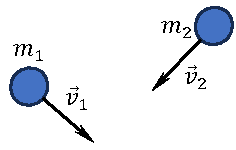
\includegraphics[width=0.5\linewidth]{image/Удар}
	\caption{Схема соударения двух тел}
	\label{fig:collision}
\end{figure}

\subsubsection{Абсолютно упругий удар}

Для сравнения приведём основные характеристики абсолютно упругого удара:

\begin{itemize}
	\item Сохранение кинетической энергии: $\frac{m_1 v_1^2}{2} + \frac{m_2 v_2^2}{2} = \frac{m_1 u_1^2}{2} + \frac{m_2 u_2^2}{2}$
	\item Сохранение импульса: $m_1\vec{v}_1 + m_2\vec{v}_2 = m_1\vec{u}_1 + m_2\vec{u}_2$
	\item Скорости после удара (1D случай):
	\[ u_1 = \frac{(m_1 - m_2)v_1 + 2m_2 v_2}{m_1 + m_2} \]
	\[ u_2 = \frac{(m_2 - m_1)v_2 + 2m_1 v_1}{m_1 + m_2} \]
\end{itemize}
	\subsection{Уравнение Бернулли}
За время $\Delta t$ жидкость течет из сечения: \(1 \to  1' \text{ и } 2 \to 2'\) (см. рис. \ref{fig:8.1.2}).

Запишем теорему об изменении механической энергии.
\[d \, W_{\text{механическая}} = d \, A^{\text{давления}}\]
\[\frac{d \, m}{2}(v_2^2 - v_1^2) + g(h_2 - h_2) d \, m = v_1 p_1 d \, S_1 \cdot d \,t_1+v_2 p_2 d \, S_2 \cdot d \,t_2\]
\[\begin{aligned}
	d m = \rho_1 v_1 d S_1 \cdot d t && &&  v_1 dS_1 = v_2 dS_2
\end{aligned}\]
\[\begin{aligned}
	\frac{\rho v_1^2}{2} + \rho g h_1 + p_1 = \frac{\rho v_2^2}{2} + \rho gh_2 + p_2 && \Rightarrow && \boxed{\frac{\rho v^2}{2} + \rho g h + p = const}
\end{aligned}\]

\textbf{Обобщение:} Выполняется вдоль линии тока\footnote{Линия тока -- линия, касательная которой в каждой точке совпадает с вектором движения}.
\begin{figure}[h]
	\centering
	\begin{minipage}{0.49\linewidth}
		\centering
		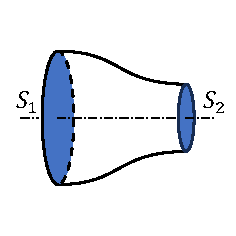
\includegraphics[width=0.7\linewidth]{image/Уравнение Бернули 2.pdf}
		\subcaption{ }
		\label{fig:8.1.1}
	\end{minipage}
	\hfill
	\begin{minipage}{0.49\linewidth}
		\centering
		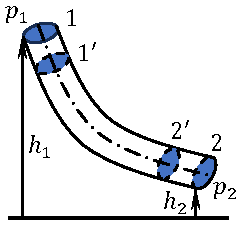
\includegraphics[width=0.7\linewidth]{image/Уравнение Бернули.pdf}
		\subcaption{ }
		\label{fig:8.1.2}
	\end{minipage}
	\caption{Пример уравнения Бернулли}
	\label{fig:bernoulli}
\end{figure}

\textbf{Пример:} (см. рис. \ref{fig:8.1.1})
\[\begin{aligned}
	\frac{\rho v_1^2}{2} + p_1 = \frac{\rho v_2^2}{2} + p_2 && (h = const)
\end{aligned}\]

Так как $S_1 > S_2$, то $v_1 < v_2$ и поэтому $p_1 > p_2$.
	\subsection{\textbf{Уравнение вращательного движения твердого тела вокруг неподвижной оси. Момент инерции, примеры его вычисления.}}
	\subsection{Теорема Гюйгенса-Штейнера}
\[\boxed{J = J_c + ma^2}\]
\begin{center}
	Момент инерции относительно произвольной оси равен сумме момента инерции относительно оси, параллельной данной и проходящей через центр масс тема, и произведению массы тела на квадрат расстояния между осями.
\end{center}
\begin{figure}[H]
	\centering
	\includegraphics[width=0.5\linewidth]{"image/Теорема Гюгенса-Штейнера"}
	\caption{Доказательство теоремы Гюгенса-Штейнера}
	\label{fig:1}
\end{figure}

\subsubsection*{Доказательство}
\vspace{-2em}
\begin{gather*}
	\vec{r_{\perp}'} = \vec{r_\perp} + \vec{a}\\
	J = \int_m {r_{\perp}'}^2 \, dm = \int_m {r_\perp}^2 \, dm + 2 \vec{a} \underbrace{\int_m \vec{r_\perp} \, dm}_{0} + a^2 \int_m \, dm = \boxed{J_c + ma^2}
\end{gather*}
\begin{center}
	\textbf{Что и требовалось доказать!}
\end{center}

Точки $O$ и $O'$ являются взаимными или сопряженными в том смысле если, подвесить маятник в точке $O'$, то центр качания будет в точке $O$, а период не изменится.

\subsubsection*{Доказательство}
\[\begin{aligned}
	l_{\text{пр}}' = r_c' + \frac{J_c}{m r_c'} = \frac{J_c}{mr_c} + r_c = l_{\text{пр}}  &&&& r_c' = \frac{J_c}{mr_c}
\end{aligned}\]
	\subsection{Кинетическая энергия и работа при вращении твердого тела вокруг неподвижной оси}
	\subsection{Кинематика плоского движения твердого тела. Мгновенная ось вращения}

\textbf{Плоское движение твердого тела} -- это движение, при котором каждая точка движется в плоскости и плоскости параллельной друг другу.
\[\vec{r} = \vec{r}_0 + \vec{r}^{\,\prime} \, \Big| \dd{}{t}\]
\[\boxed{\vec{v} = \vec{v}_0 + [\vec{\omega}; \, \vec{r}^{\,\prime}]}\]
\begin{center}
	Математическое выражение плоского движения.
\end{center}
\begin{figure}[h]
	\centering
	\begin{minipage}{0.49\linewidth}
		\centering
		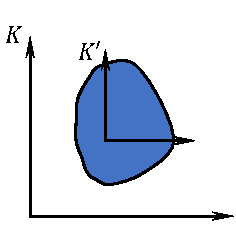
\includegraphics[width=0.6\linewidth]{image/Кинематика Плоского Движения.pdf}
		\subcaption{ }
		\label{fig:12.1.1}
	\end{minipage}
	\hfill
	\begin{minipage}{0.49\linewidth}
		\centering
		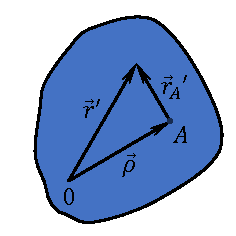
\includegraphics[width=0.6\linewidth]{image/Кинематика Плоского Движения 1.pdf}
		\subcaption{ }
		\label{fig:12.1.2}
	\end{minipage}
	\caption{Иллюстрации к вопросу}
	\label{fig:5}
\end{figure}

Возьмем разные полюса. Будет ли $\omega$ зависеть от выбора полюса?
\begin{align*}
	&\vec{v}=\vec{v}_0+ [\vec{\omega}; \, \vec{r}^{\, \prime}] \\
	&\vec{v}=\vec{v}_A+[\vec{\omega}_A; \, \vec{r}^{\, \prime}_A] \\
	& \vec{v}_0+ [\vec{\omega}; \, \vec{r}^{\, \prime}] = \vec{v}_A+[\vec{\omega}_A; \, \vec{r}^{\, \prime}_A]\\
	&\vec{v}_A = \vec{v}_0 + [\vec{\omega}; \, \vec{\rho}] \text{ -- т.к. точка $A$ вращается вокруг $O$}\\
	& \vec{v}_0+ [\vec{\omega}; \, \vec{r}^{\, \prime}] = \vec{v}_0+[\vec{\omega}; \, \vec{\rho}]+[\vec{\omega}_A; \, \vec{r}^{\, \prime}_A] \\
	& [\vec{\omega}; \, (\vec{r}^{\, \prime} - \vec{\rho})] = \vec{v}_0+[\vec{\omega}; \, \vec{\rho}]+[\vec{\omega}_A; \, \vec{r}^{\, \prime}_A] \\
	& [\vec{\omega}; \, (\vec{r}^{\, \prime} - \vec{\rho})] = [\vec{\omega}_A; \, \vec{r}^{\, \prime}_A] \\
	& \begin{aligned}
		\left.\begin{matrix}
			\vec{r}^{\,\prime} = \vec{\rho} + \vec{r}_A^{\, \prime} \\
			\vec{r}^{\,\prime} - \vec{\rho} = \vec{r}_A^{\,\prime}
		\end{matrix} \, \right|
		\Rightarrow [\vec{\omega}; \, \vec{r}_A^{\,\prime}] = [\vec{\omega}_A; \, \vec{r}_A^{\,\prime}]
	\end{aligned}
\end{align*}

В общем случае $\vec{\omega} \neq \vec{\omega}_A$, но в случае плоского движения $\vec{\omega}_A = \vec{\omega}$.

\textbf{Вывод:} Угловая скорость вращения носит абсолютный характер, то есть можно не указывать ось вращения. Часто за полюс берут центр масс.
\[\vec{v} = \vec{v} + [\vec{\omega}; \, \vec{r}^*]\]
где $\vec{r}^*$ -- радиус-вектор от центра масс до произвольной точки.

\subsubsection*{Мгновенная ось вращения}

\textbf{Мгновенная ось вращения} -- это ось, связанная с точкой тела, у которой скорость равна нулю ($\vec{v} = 0$) в данный момент времени. Такую точку всегда можно найти:
\[\vec{v} = \vec{v}_c + [\vec{\omega}; \, \vec{r}_M^{\,*}] = 0 \, \Big| \cdot \vec{\omega}\]
\[[\vec{\omega}; \, \vec{v}_c] + [\vec{\omega}; \, [\vec{\omega}; \, \vec{r}_M^{\, *}]] = 0\]
\[[\vec{\omega}; \, \vec{v}_c] + \omega\underbrace{(\vec{\omega}; \, \vec{r}_M^{\,*})}_{0} - \vec{r}_M^{\,*} \vec{\omega}^2 = 0\]
\[\begin{aligned}
	\vec{r}_M^{\,*} = \frac{[\vec{\omega}; \, \vec{v}_c]}{\omega^2} &&\to&& \vec{r}_M^{\,*} = \frac{v_c}{\omega}
\end{aligned}\]

\textbf{Пример:} Цилиндр без проскальзывания движется по плоскости. (см. рис. \ref{fig:7}) \textbf{Важно!} Понятие Мгновенной Оси Вращения нельзя использовать для поиска распределения ускорения.
\begin{figure}[H]
	\centering
	\includegraphics[width=0.6\linewidth]{"image/Кинематика Плоского Движения 3"}
	\caption{Пример}
	\label{fig:7}
\end{figure}



	\subsection{\textbf{Уравнения динамики плоского движения твердого тела.} Кинетическая энергия твердого тела при плоском движении}
	\subsection{\textbf{Приближенная теория гироскопа. Прецессия гироскопа.}}
	\subsection{Распределение молекул по объёму сосуда в отсутствие внешних силовых полей. Флуктуации числа молекул}
	\subsection{\textbf{Распределение Максвелла по проекции и вектору скорости}}
	\subsection{\textbf{Распределение Максвелла по модулю скорости.} Наиболее вероятная, средняя и средняя квадратичная скорости}
\begin{figure}
	\centering
	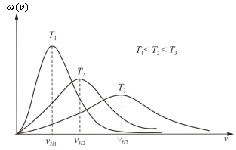
\includegraphics[width=0.5\linewidth]{image/Максвел}
	\caption{Распределение Максвелла по модулю скорости}
	\label{fig:11}
\end{figure}

\subsubsection*{Распределение Максвелла по модулю скорости}
\textbf{Задача: }Найти плотность вероятности $\omega(v)$, которая определяет вероятность того, что скорость молекулы находится в интервале $[v; \, v + dv]$.
\begin{align} \label{17.1}
	\boxed{\omega(v) = 4 \pi v^2 \left(\frac{m}{2\pi k T}\right)^{\frac{3}{2}} \exp \left(-\frac{mv^2}{2kT}\right)}
\end{align}

\[\int_{0}^{\infty} \omega(v) \, dv = 1\]

\textbf{Наиболее вероятный исход }-- это скорость, при которой функция распределения достигает максимума.
\begin{align*}
	v_\text{вер.} = \sqrt{\frac{2RT}{\mu}} && \langle v \rangle = \int_{0}^{\infty} v \cdot \omega(v) \, dv = \sqrt{\frac{8kT}{\pi m}}
\end{align*}

\textbf{Среднеквадратичная скорость:}
\begin{align*}
	v_\text{кв} = \sqrt{\langle v^2 \rangle} && \langle v^2 \rangle = \int_{0}^{\infty} v^2 \omega(v) \, dv = \frac{3kT}{m}
\end{align*}
\[\langle v^2 \rangle = \langle v^2_x \rangle + \langle v^2_y \rangle + \langle v^2_z \rangle = \frac{3kT}{m}\]

\textbf{Среднеквадратичная скорость} определяет среднюю кинетическую энергию:
\begin{align*}
	\langle W_\text{кин} \rangle = \langle \frac{mv^2}{2} \rangle = \frac{m}{2} \langle v^2 \rangle = \frac{mv^2_\text{кв}}{2} = \frac{3}{2}kT && \boxed{\langle W_\text{кин} \rangle = \frac{3}{2}kT}
\end{align*}
	\subsection{\textbf{Распределение Больцмана}, барометрическая формула}
	\subsection{Давление идеального газа. \textbf{Уравнение Клапейрона-Менделеева}}
	\subsection{Внутренняя энергия идеального газа и ее связь с температурой.}
	\subsection{Средняя длина свободного пробега молекул в газах}

\textbf{Средняя длина свободного пробега} - это среднее расстояние, проходимое молекулой между двумя соударениями. Обозначается как $\lambda \, [\text{м}]$.

\begin{table}[h]
	\centering
	\caption{Эффективные диаметры атомов и молекул в газовой фазе}
	\begin{tabular}{|c|c|c|}
		\hline
		\textbf{Элемент} & \textbf{Символ} & \textbf{Эффективный диаметр, \( d \, (\mathring{A})\) } \\
		\hline
		Гелий & He & 2,0 \\
		Неон & Ne & 2,2 \\
		Аргон & Ar & 3,6 \\
		Криптон & Kr & 4,0 \\
		Ксенон & Xe & 4,5 \\
		Радон & Rn & 5,0 \\
		\hline
		Водород & H\textsubscript{2} & 2,4 \\
		Азот & N\textsubscript{2} & 3,7 \\
		Кислород & O\textsubscript{2} & 3,5 \\
		Углекислый газ & CO\textsubscript{2} & 4,6 \\
		\hline
	\end{tabular}
	\label{tab:diameters}
\end{table}

Будем считать что все молекулы кроме одной неподвижны. Среднее расстояние проходимое молекулой за время $t$ тогда будет равно:
\[
L = \langle v\rangle \cdot t \quad \text{и} \quad V = \pi d^2 L = \pi d^2 \langle v \rangle t
\]

Среднее \textit{число соударений}:
\[
z = Vn = \pi d^2 n \langle v\rangle t
\]

Средняя \textit{частота соударения}:
\[
\vartheta = \frac{z}{t} = \pi d^2 n \langle v \rangle
\]

Средняя \textit{длина свободного пробега}:
\[
\lambda = \frac{\langle v \rangle}{\vartheta} = \frac{1}{\pi d^2 n}
\]

Если учитывать движение всех молекул, то:
\[
\vartheta = \sqrt{2} \pi d^2 n \langle v \rangle = \sqrt{2}\sigma n \langle v \rangle, \quad \text{где } \sigma = \pi d^2
\]
\[
\lambda = \frac{1}{\sqrt{2} \pi d^2 n} = \frac{1}{\sqrt{2} \sigma n}
\]

При нормальных условиях концентрация равна:
\[
n = N_L = 2,\!7 \times 10^{19} \text{ см}^{-3}
\]
\[
\lambda \approx 1,\!7 \times 10^{-5} \text{ см} = 170 \text{ нм}
\]
\[
\langle v \rangle \approx 10^{-1} \, \text{км/с}
\]
\[
\tau = \frac{1}{\vartheta} \approx 10^{-9} \text{ с}
\]

За это время устанавливается распределение Максвелла.

\begin{tbox}{Распределение Максвелла}
	\textbf{Распределение Максвелла} описывает распределение молекул газа по скоростям в условиях термодинамического равновесия. Для идеального газа вероятность того, что молекула имеет скорость в интервале от $v$ до $v+dv$, задаётся функцией:

	\[
	f(v) = 4\pi \left(\frac{m}{2\pi k T}\right)^{3/2} v^2 \exp\left(-\frac{mv^2}{2k T}\right)
	\]

	где:
	\begin{itemize}
		\item $m$ — масса молекулы
		\item $k$ — постоянная Больцмана ($1,380649 \times 10^{-23} \, \frac{\text{Дж}}{\text{К}}$)
		\item $T$ — абсолютная температура
		\item $v$ — скорость молекулы
	\end{itemize}

	Характерные скорости:
	\begin{enumerate}
		\item \textbf{Наиболее вероятная скорость} (соответствует максимуму распределения):
		\[
		v_{\text{вер}} = \sqrt{\frac{2k_B T}{m}}
		\]

		\item \textbf{Средняя скорость}:
		\[
		\langle v \rangle = \sqrt{\frac{8k_B T}{\pi m}}
		\]

		\item \textbf{Среднеквадратичная скорость}:
		\[
		v_{\text{ск}} = \sqrt{\frac{3k_B T}{m}}
		\]
	\end{enumerate}

	Соотношение между характерными скоростями:
	\[
	v_{\text{вер}} : \langle v \rangle : v_{\text{ск}} = 1 : \sqrt{\frac{4}{\pi}} : \sqrt{\frac{3}{2}} \approx 1 : 1,128 : 1,225
	\]

	За время порядка $\tau \approx 10^{-9}$ с после соударения устанавливается распределение Максвелла.
\end{tbox}
	\subsection{Диффузия в газах. Закон Фика, расчёт коэффициента диффузии}
	\subsection{Внутреннее трение в газах. Формула Ньютона, расчет вязкости}
	\subsection{Теплопроводность в газах. Закон Фурье, расчет коэффициента теплопроводности}

\textbf{Теплопроводность} -- это явление возникновения потока тепла в неравномерно нагретой среде, обусловленное передачей энергии от более нагретых участков к менее нагретым за счет теплового движения и взаимодействия частиц (атомов, молекул, электронов).
	\subsection{Броуновское движение. Формула Эйнштейна}
\subsubsection*{Броуновское движение}
\textbf{Броуновское движение} - это непрерывное хаотическое движение макроскопических частиц в жидкости или газе, вызванное ударами молекул окружающей среды.

Частица образует с молекулами газа единую систему \textbf{ТРРЭПСС} (термодинамически равновесную систему с равномерно распределённой энергией по степеням свободы).

Будем считать, что смещения статистически независимы: смещение от $0$ до $t_1$ и от $t_1$ до $t$ ничего не дает в корреляции.
\begin{gather*}
	\langle x^2 \rangle = \langle x_1^2\rangle + \langle x_2^2\rangle\\
	\langle x^2 \rangle = f(t) \\
	\begin{aligned}
		\langle x_1^2 \rangle = f(t_1) && \langle x_2^2 \rangle = f(t - t_1)
	\end{aligned}\\
	f(t) = f(t_1) + f(t - t_1)
\end{gather*}

Единственное решение, удовлетворяющее этому функциональному уравнению - линейная зависимость:
\begin{align*}
	f(t) = \alpha t && \text{где } \alpha = \text{const}
\end{align*}

Таким образом получаем:
\begin{align*}
	\langle x^2 \rangle = \alpha t && \langle x^2\rangle = \langle y^2\rangle = \langle z^2 \rangle = \alpha t
\end{align*}


\subsubsection*{Формулы Эйнштейна}
Уравнение Ланжевена для броуновской частицы:
\[ m\ddot{x} = -h\dot{x} + F_x(t) \quad \Big|\cdot x \]
где:
\begin{itemize}
	\item $m$ — масса частицы [кг]
	\item $h$ — коэффициент трения [кг/с]
	\item $F_x(t)$ — случайная сила [Н]
	\item $x$ — координата частицы [м]
\end{itemize}

\[ mx\ddot{x} = -hx\dot{x} + xF_x(t) \]

Используем тождества для производных:
\[ \frac{d}{dt}(x^2) = 2x\dot{x}, \quad \frac{d^2}{dt^2}(x^2) = 2\dot{x}^2 + 2x\ddot{x} \]

Выражаем $x\ddot{x}$:
\[ x\ddot{x} = \frac{1}{2}\frac{d^2}{dt^2}x^2 - \dot{x}^2 \]

Подставляем в уравнение:
\[ \frac{m}{2}\frac{d^2}{dt^2}x^2 - m\dot{x}^2 = -\frac{h}{2}\frac{d}{dt}x^2 + xF_x(t) \]

Усредняем:
\[ \frac{m}{2}\frac{d^2}{dt^2}\langle x^2\rangle - \langle m\dot{x}^2\rangle = -\frac{h}{2}\frac{d}{dt}\langle x^2\rangle + \langle xF_x(t)\rangle \]

Учитываем:
\begin{itemize}
	\item $\langle m\dot{x}^2\rangle = kT$ [Дж], где $k$ — постоянная Больцмана [Дж/К], $T$ — температура [К]
	\item $\langle xF_x(t)\rangle = 0$ [Н·м]
\end{itemize}

Для стационарного режима ($t \gg m/h$):
\[ -kT = -\frac{h}{2}\frac{d}{dt}\langle x^2\rangle \]

Получаем:
\[ \frac{d}{dt}\langle x^2\rangle = \frac{2kT}{h} \quad \text{[м$^2$/с]} \]

Интегрируем:
\[ \langle x^2\rangle = \frac{2kT}{h}t = \frac{kT}{3\pi\eta a}t \quad \text{[м$^2$]} \]
где $\eta$ — вязкость жидкости [Па·с], $a$ — радиус частицы [м]

Для трехмерного случая:
\[ \langle r^2\rangle = \frac{kT}{\pi\eta a}t \quad \text{[м$^2$]} \]

Итоговые формулы:
\[ \boxed{\langle x^2\rangle = \frac{kT}{3\pi\eta a}t \quad [\text{м}^2]}, \quad \boxed{\langle r^2\rangle = \frac{kT}{\pi\eta a}t \quad [\text{м}^2]} \]
	\subsection{Классическая теория теплоемкости газов. Теорема о равнораспределении энергии по степеням свободы. Недостатки классической теории теплоемкости}
	\subsection{Общий и нулевой принципы термодинамики. Измерение температуры. Классификация процессов}
	\subsection{\textbf{Первый принцип термодинамики. Внутренняя энергия идеального газа. Примеры применения: соотношение Майера, уравнение адиабатического процесса}}
	\subsection{\textbf{Второй принцип термодинамики. Формулировки для тепловых двигателей и холодильных машин}}
	\subsection{\textbf{Цикл Карно и его КПД.} Первая теорема Карно}
	\subsection{Необратимые циклы, вторая теорема Карно}
	\subsection{Уравнение Ван-дер-Ваальса. Фазовые переходы.}
	\subsection{Внутренняя энергия газа Ван-дер-Ваальса.}
	\subsection{Приведенное количество теплоты. Равенство Клаузиуса. Энтропия. Энтропия идеального газа.}

\textbf{Определение: } $\dfrac{dQ}{T}$ -- элементарная приведенная количество тепла. Где $T$ -- температура теплового резервуара, с которым газ обеспечивается теплом. Для обратимых процессов совпадает с температурой газа.

\subsubsection*{Равенство Клаузиуса. II принцип термодинамики для обратимых процессов}
\begin{figure}[H]
	\centering
	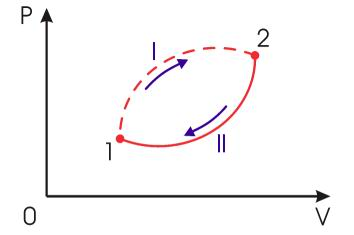
\includegraphics[width=0.7\linewidth]{image/Rule}
	\caption{График $pV$-диаграммы.
		Кривые I и II представляют разные термодинамические процессы между состояниями 1 и 2.}
	\label{fig:9}
\end{figure}
Из его равенства вытекает важное следствие. Приведенное количество теплоты при конечном обратимом переходе не зависит от пути, а зависит от:
\begin{align} \label{34.1}
	\boxed{\oint \frac{dQ}{T} = 0}
\end{align}
\begin{align} \label{34.2}
	\int\limits_{1\,I\,2} \frac{dQ}{T} + \int\limits_{2\,II\,1} \frac{dQ}{T} = 0
\end{align}

Математическая формула II принципа термодинамики для обратных процессов.

\begin{tbox}{ВАЖНО!}
	Существует такая функция состояния системы ее энтропии $S$, что разность значений этой функции в состояниях $1$ и $2$ ($S_1$ и $S_2$) равна:
	\begin{align} \label{34.3}
		S_2 - S_1 = \int_{1}^{2}\frac{dQ}{T}
	\end{align}
	\begin{center}
		\textit{(для обратимых процессов)}
	\end{center}
\end{tbox}

\subsubsection*{Энтропия идеального газа}
\begin{figure}[H]
	\centering
	\includegraphics[width=0.4\linewidth]{"image/Энтропия идеального газа"}
	\caption{Энтропия идеального газа}
	\label{fig:10}
\end{figure}

Запишем I принцип термодинамики и определение энтропии:
\begin{align*}
	dS = \frac{dQ}{T} && \begin{aligned}
		dQ = dU + dA' = \vartheta C_{\vartheta} dT + pdV = \\
		= \vartheta C_\vartheta dT + \vartheta RTdV
	\end{aligned}
\end{align*}
\[dS = \frac{\vartheta C_\vartheta dT}{T} + \vartheta R dV\]
\[S = \vartheta C_\vartheta \ln T + \vartheta R \ln V + const\]
\[S = \vartheta C_\vartheta (\ln T + \frac{R}{C_\vartheta} \ln V) + const\]

Пусть $\frac{R}{C_\vartheta} = \gamma - 1$:
\begin{align} \label{34.4}
	\boxed{S = \vartheta C_\vartheta \ln (T V^{\gamma - 1}) + const} && \boxed{S = \vartheta C_\vartheta \ln (p V^{\gamma}) + const}
\end{align}

	\subsection{Неравенство Клаузиуса. Закон возрастания энтропии (с примерами).}

	%\section*{Физика}
\begin{multicols}{2}
	\noindent
	\subsection*{Механика}
	\begin{enumerate}[leftmargin=*,itemsep=0cm,parsep=0cm]
		\item $\square$ \textbf{Теорема об изменении импульса с.м.т.} Условия сохранения импульса.
		\item $\square$ \textbf{Теорема о движении центра масс.}
		\item $\square$ Уравнение Мещерского. Реактивная сила.
		\item $\square$ \textbf{Теорема об изменении момента импульса с.м.т.} Закон сохранения момента импульса.
		\item $\square$ \textbf{Теорема об изменении кинетической энергии с.м.т.}
		\item $\square$ Потенциальная энергия с.м.т. \textbf{Теорема об изменении механической энергии с.м.т. Условия сохранения механической энергии.}
		\item $\square$ Абсолютно неупругое/упругое соударение частиц.
		\item $\square$ Уравнение Бернулли.
		\item $\square$ \textbf{Уравнение вращательного движения твёрдого тела. Момент инерции.}
		\item $\square$ Теорема Гюйгенса-Штейнера.
		\item $\square$ Кинетическая энергия и работа при вращении твердого тела вокруг неподвижной оси.
		\item $\square$ Кинематика плоского движения твердого тела. Мгновенная ось вращения.
		\item $\square$ \textbf{Уравнения динамики плоского движения твердого тела.} Кинетическая энергия твердого тела при плоском движении.
		\item $\square$ \textbf{Приближенная теория гироскопа. Прецессия гироскопа.}
	\end{enumerate}
	\subsection*{Молекулярная физика и термодинамика}
	\begin{enumerate}[leftmargin=*,itemsep=0cm,parsep=0cm,start=15]
		\item $\square$ Распределение молекул по объёму сосуда в отсутствие внешних силовых полей. Флуктуации числа молекул.
		\item $\square$ \textbf{Распределение Максвелла по проекции и вектору скорости. }
		\item $\square$ \textbf{Распределение Максвелла по модулю скорости.} Наиболее вероятная, средняя и средняя квадратичная скорости.
		\item $\square$ Распределение Больцмана, барометрическая формула.
		\item $\square$ Давление идеального газа. Уравнение Клапейрона-Менделеева.
		\item $\square$ Внутренняя энергия идеального газа и ее связь с температурой.
		\item $\square$ Средняя длина свободного пробега молекул в газах.
		\item $\square$ Диффузия в газах. Закон Фика, расчёт коэффициента диффузии.
		\item $\square$ Внутреннее трение в газах. Формула Ньютона, расчет вязкости.
		\item $\square$ Теплопроводность в газах. Закон Фурье, расчет коэффициента теплопроводности.
		\item $\square$ Броуновское движение. Формула Эйнштейна.
		\item $\square$ Классическая теория теплоемкости газов. Теорема о равнораспределении энергии по степеням свободы. Недостатки классической теории теплоемкости.
		\item $\square$ Общий и нулевой принципы термодинамики. Измерение температуры. Классификация процессов.
		\item $\square$ \textbf{Первый принцип термодинамики. Внутренняя энергия.}
		\item $\square$ \textbf{Второй принцип термодинамики. Формулировки.}
		\item $\square$ Цикл Карно и его КПД. Теоремы Карно.
		\item $\square$ Уравнение Ван-дер-Ваальса. Фазовые переходы.
		\item $\square$ Внутренняя энергия газа Ван-дер-Ваальса.
		\item $\square$ Приведенное количество теплоты. Равенство Клаузиуса. Энтропия. Энтропия идеального газа.
		\item $\square$ Неравенство Клаузиуса. Закон возрастания энтропии (с примерами).
	\end{enumerate}
\end{multicols}

	\thispagestyle{empty}
\begin{center}
	\vspace*{\fill}

	\begin{tcolorbox}[
		width=0.7\textwidth,
		colback=white,
		colframe=black!50,
		arc=4mm,
		boxrule=1pt,
		enhanced jigsaw
		]
		\centering
		{\LARGE \textbf{Скороходов Сергей Александрович}} \\[0.5cm]
		{\large \textit{Студент 1 курса}} \\[1cm]

		\begin{tabular}{ll}
			\textbf{Email:} & \href{mailto:sergey.skor007@gmail.com}{sergey.skor007@gmail.com} \\
			\textbf{Telegram:} & \href{https://t.me/SerKin0}{t.me/SerKin0} \\
			\textbf{GitHub:} & \href{https://github.com/SerKin0}{github.com/SerKin0} \\
			\textbf{VK:} & \href{https://vk.com/serking2}{vk.com/serking2}
		\end{tabular}
	\end{tcolorbox}

	\vspace*{\fill}
\end{center}
\end{document}